% Preamble
\documentclass[11pt]{article}

% Packages
\usepackage{amsmath}
\usepackage{mathtools}
\usepackage{ragged2e}
\usepackage [utf8]{inputenc}
\usepackage{blindtext}
\usepackage{wrapfig}
\usepackage{xcolor}
\usepackage {polski}
\usepackage{multicol}
\usepackage[a4paper, total={5.7in, 8in}]{geometry}
\usepackage{graphicx}
\usepackage{amstex}
\usepackage{csvsimple}
\usepackage{changepage}
\usepackage{enumitem}
\usepackage[english]{babel}
\usepackage{biblatex}
\usepackage{caption}
\usepackage{indentfirst}
\usepackage{epstopdf-base}
\usepackage{textcomp}
\usepackage{wasysym}

% Document
\begin{document}
%    Nagłówek
    \begin{flushleft}
        Maciej Pierzchała 282 934 \hfill Data wykonania ćwiczenia:\\
        Filip Kubecki 272 655 \hfill 5 listopada 2024r\\
        Grupa: Wtorek 10:35 \\
    \end{flushleft}
    \begin{center}
        \Large\textbf{Laboratorium 4}\\
        \textbf{Charakteryzacja czujników alkoholu}
    \end{center}
    \hfill
%    Treść
    \section{Spis przyrządów}
    \par{
        Do wykonania ćwiczenia wykorzystano:
        \begin{itemize}
            \setlength\itemsep{0em}
            \item[-] Multimetr cyfrowy Sigilent SDM 3055
            \item[-] Termohigrobarometr LAB-EL LB706B
            \item[-] Rezystancyjny czujnik alkoholu
            \item[-] Amperometryczny czujnik alkoholu
            \item[-] Kolby zawierające odpowiednie stężenia alkocholu oraz acetonu
        \end{itemize}
    }
    \section{Przebieg i cele doświadczenia}
    \par Doświadczenie miało na celu zapoznać nas z zasadami działania różnych typów czujników alkoholu.
    \indent Celami doświadczenia było wyznaczenie krzywych kalibracyjnych dla rezystancyjnego oraz amperometrycznego czujnika alkoholu,
    oraz obliczenie nieznanej koncentracji alkocholu w kolbie "X" na podstawie tych krzywych.

    \section{Obliczenia i analiza wyników}
    \par Wykorzystując dane pomiarowe przekształcono zmierzone rezystancję na konduktancje przy pomocy poniższego wzoru:
    \begin{gather}
        G=\frac{1}{R}
    \end{gather}
    \noindent Przykładowo dla pomiaru dla wartości $60 [ppm]$:
    \begin{gather}
        G=\frac{1}{7.27[k\Omega]}=0.00013755158[S]\approx137.552[\mu S]
    \end{gather}
    \noindent Przy pomocy obliczonych wartości konduktancji wyznaczono czułość czujnika dla odpowiednich atmosfer ze wzoru:
    \begin{gather}
        S=\frac{G_{gaz}}{G_0}
    \end{gather}
        \noindent Gdzie:
        {\footnotesize
    \begin{itemize}
        \setlength\itemsep{0em}
        \item[] \textbf{$G_{gaz}$} - konduktancja w atmosferze pomiaru,
        \item[] \textbf{$G_0$} - konduktancja w atmosferze zerowej/otoczenia,
    \end{itemize}}
    \noindnet Przykładowo dla pomiaru w atmosferze $60 [ppm]$:
    \begin{gather}
        S=\frac{137.552[\mu S]}{29.586[\mu S]}=4.649225
    \end{gather}
    \noindent Wszystkie wyniki Konduktancji oraz czułości znajdują się wa Tabeli 1.\\
    \indent Na podstawie wyliczonych konduktancji oraz czułości wyznaczono krzywą kalibracyjną czujnika ($G=f(x)$) oraz krzywą $S=f(x)$:\\
    \noindent\makebox[\textwidth]{
        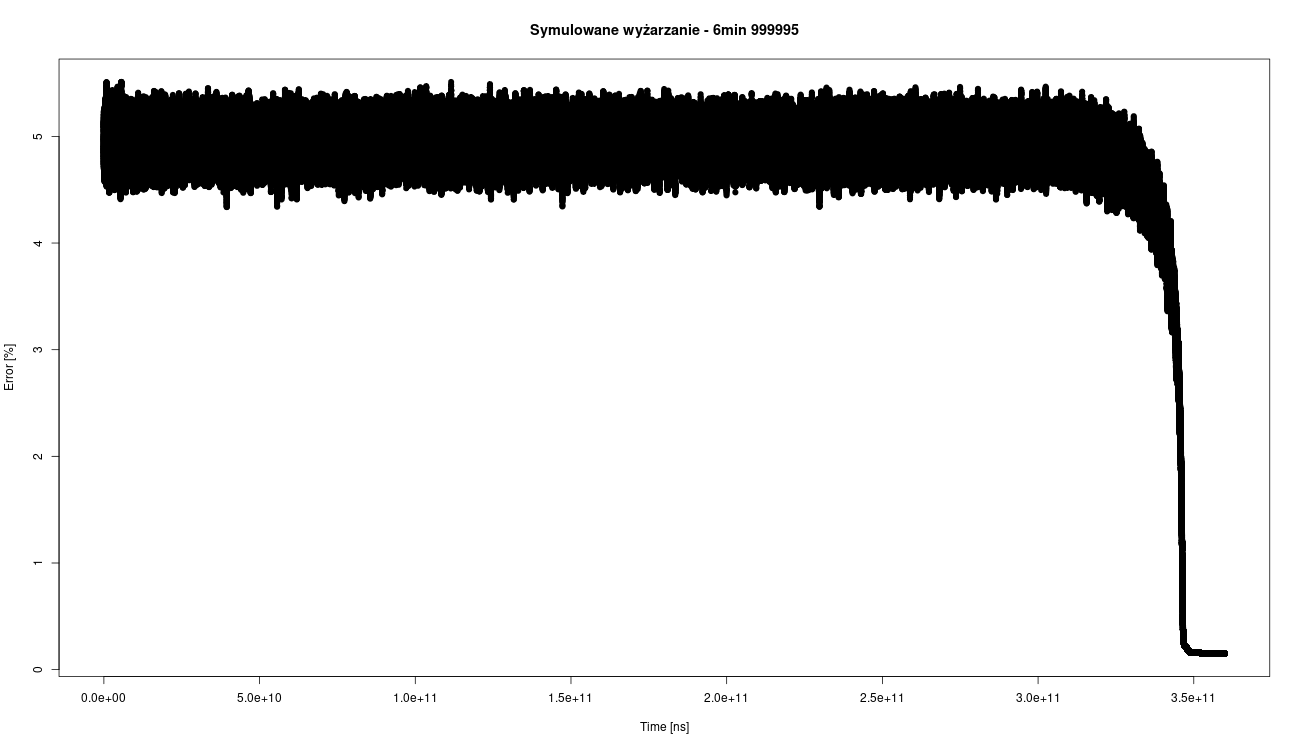
\includegraphics[scale = 0.35]{/home/bork/IdeaProjects/LatexProjects/src/PodstawyTechnikiSensorowej/Lab4/Img/resistanceG=f(x)}}
    \noindent\makebox[\textwidth]{
        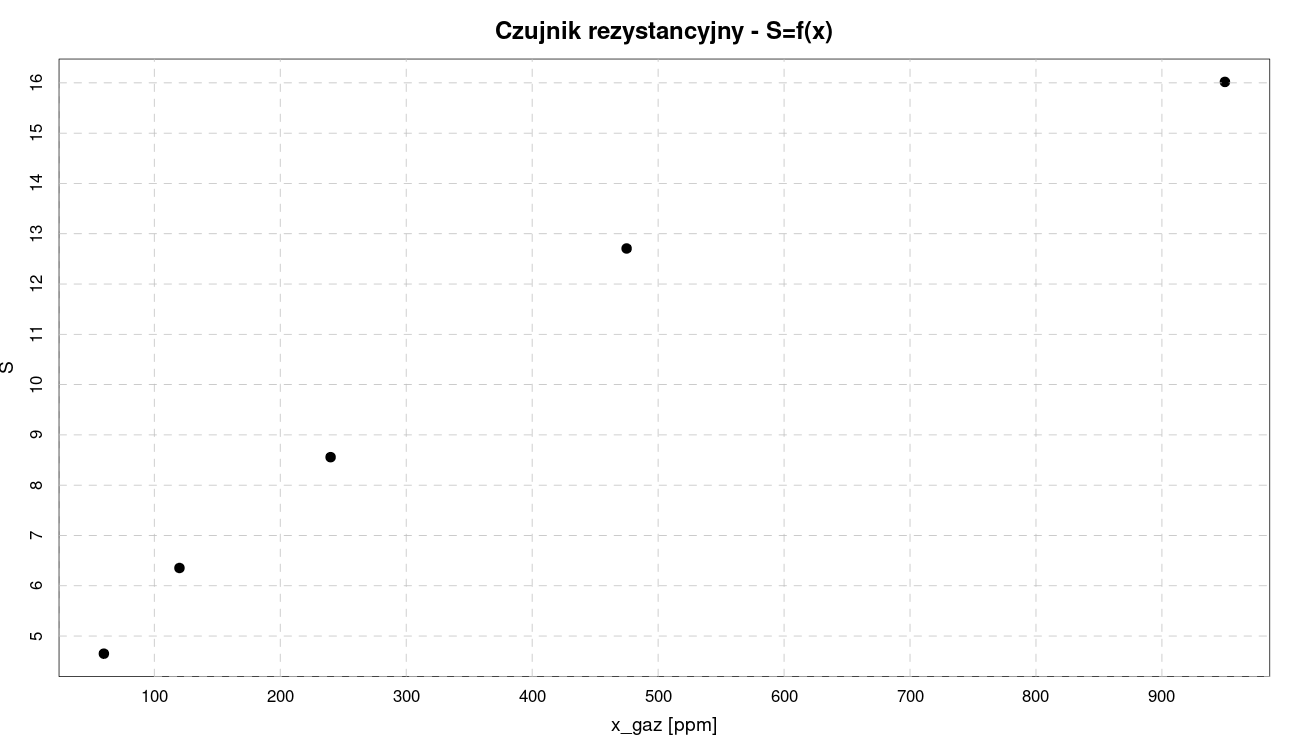
\includegraphics[scale = 0.35]{/home/bork/IdeaProjects/LatexProjects/src/PodstawyTechnikiSensorowej/Lab4/Img/resistanceS=f(x)}}
    \indent Wykorzystując język programowania R wyznaczono metodą regresji logarytmicznej współczynniki dla krzywej aproksymującej krzywą kalibracyjną
    $G=f(x)$. Wynik kalkulacji oraz krzywa wyznaczona na podstawie regresji logarytmicznej zostały przedstawione na wykresie $G=f(x)$.\\
    \indent Przekształcając równanie funkcji aproksymującej krzywą kalibracji możemy wyznaczyć wartość stężenia alkocholu w kolbie "X".
    \begin{gather}
        y=intercept+slope\cdot \ln(x)
    \end{gather}
\noindent Gdzie:
    {\footnotesize
\begin{itemize}
    \setlength\itemsep{0em}
    \item[] \textbf{$intercept$} - punkt przecięcia z osią Y - wynikający z regresji,
    \item[] \textbf{$slope$} - nachylenie - wynikające z regresji,
    \item[] \textbf{$x$} - stężenie cząsteczek alkocholu (w [ppm]),
    \item[] \textbf{$y$} - konduktancja pomiaru (w [S] - Siemensach),
\end{itemize}}
    \begin{gather}
        y=intercept+slope\cdot \ln(x)\\
        y-intercept=slope\cdot \ln(x)\\
        \frac{y-intercept}{slope}=\ln(x)\\
        x=\exp(\frac{y-intercept}{slope})
    \end{gather}
    \indent Wyliczamy stężenie dla wartości z kolby "X":
    \begin{gather}
        x=\exp(\frac{0.0003058104+0.000397}{0.000125})=276.5753[ppm]
    \end{gather}
    \indent Dla czujnika amperometrycznego wyznaczono wartości maksymalnego natężenia prądu
    sczytując je z wyświetlacza multimetru i notując w tabeli pomiarowej. Na podstawie tych pomiarów
    stworzono wykres $i_{max}=f(x)$.\\
    \noindent\makebox[\textwidth]{
        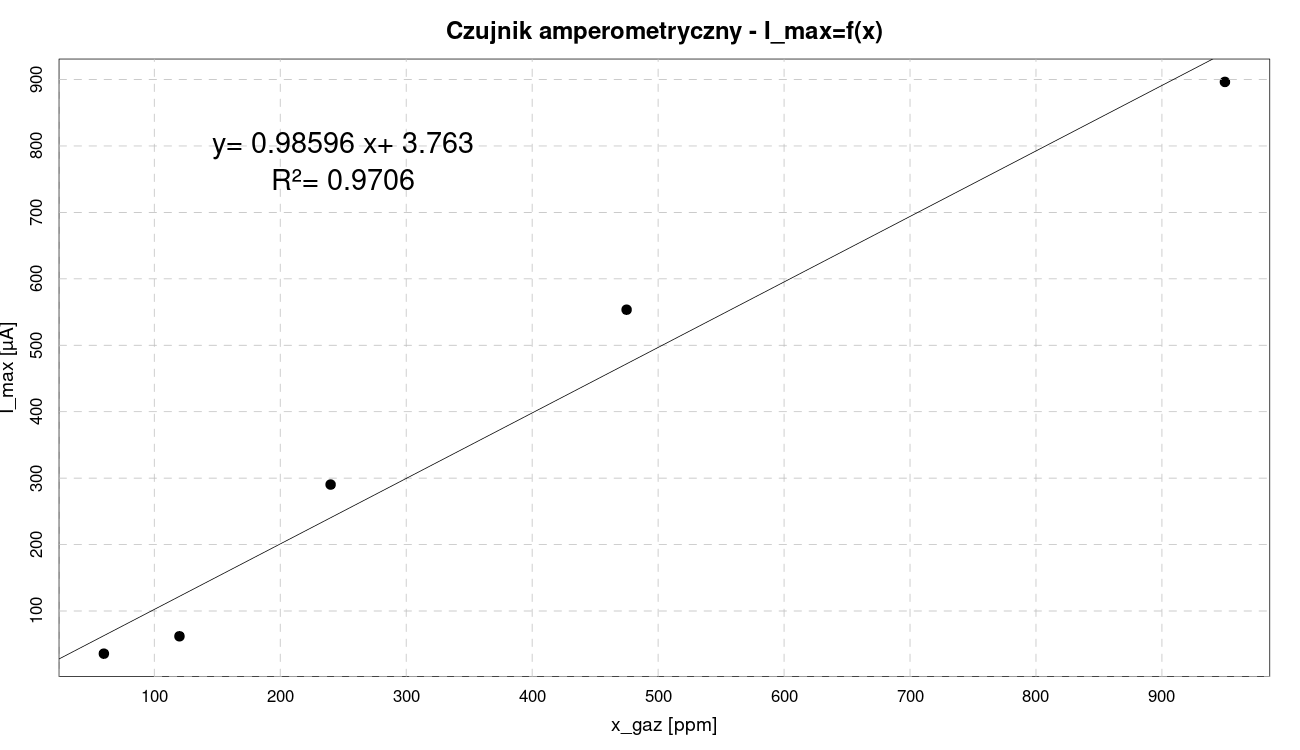
\includegraphics[scale = 0.35]{/home/bork/IdeaProjects/LatexProjects/src/PodstawyTechnikiSensorowej/Lab4/Img/amperometricimax=f(x)}}
    \indent Przy pomocy regresji liniowej wyznaczono równanie prostej aproksymującej charakterystykę naszego czujnika. Równanie to podano na
    wykresie powyżej. Przekształcając równanie prostej możemy wyznaczyć wzór na wartość x (zawartość alkocholu):
    \begin{gather}
        y=ax+b \\
        y-b=ax \\
        x=\frac{y-b}{a}
    \end{gather}
    \noindent Dla wartości zmierzonej dla kolby "X":
    \begin{gather}
        x=\frac{235.3-3.763}{0.98596}=234.8329[ppm]
    \end{gather}
    \newpage
    \indent Dla jednego pomiaru czujnikiem rezystancyjnym wyznaczono czas odpowiedzi i powrotu:\\
    \noindent\makebox[\textwidth]{
        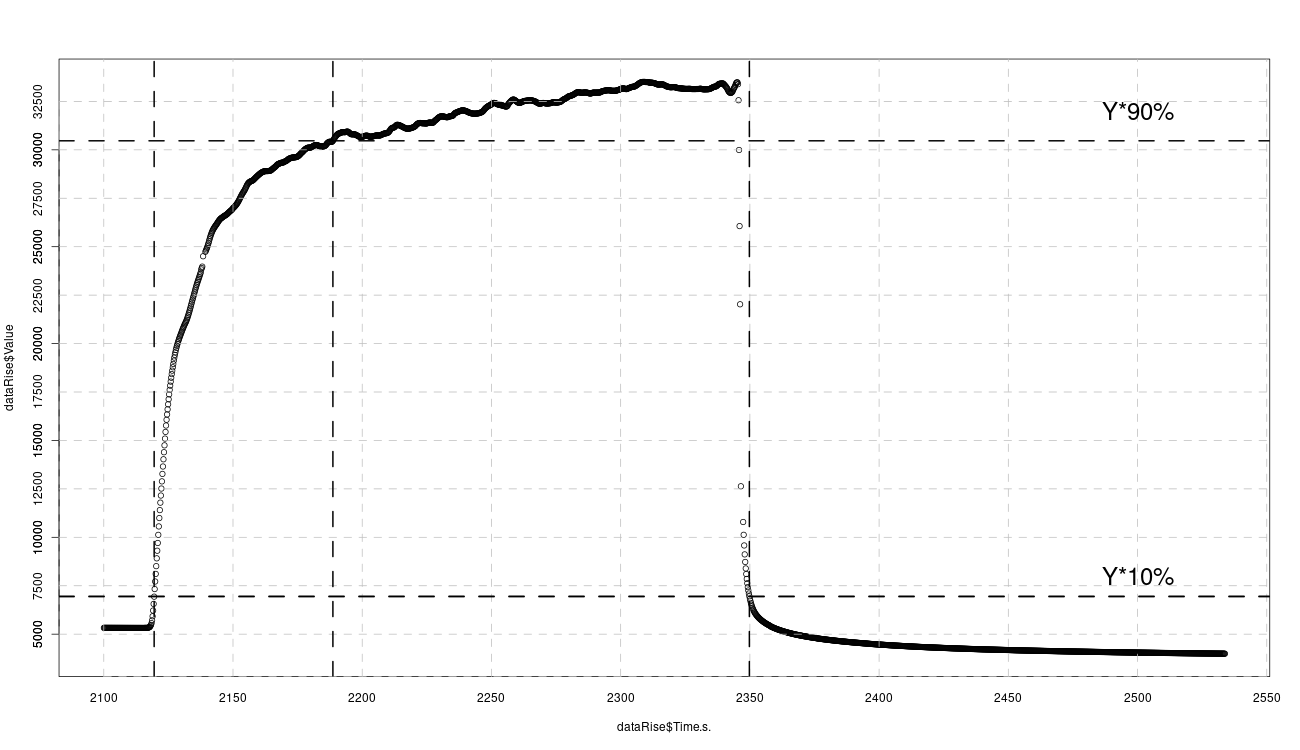
\includegraphics[scale = 0.35]{/home/bork/IdeaProjects/LatexProjects/src/PodstawyTechnikiSensorowej/Lab4/Img/resistanceSlope}}
    \begin{gather*}
        T_{rise}=52.54[s]\\
        T_{fall}=3.99[s]
    \end{gather*}
    \subsection{Tabela 1}
    \begin{center}
        \Large\csvreader[tabular = |c|c|c|c|c|,
            table head = \hline  \textbf{$x_{gaz}[ppm]$}  & \textbf{$R[k\Omega]$} & \textbf{$I_{max}[\mu A]$}  & \textbf{$G[S]$} & \textbf{$S$}  \\\hline,
            late after line = \\\hline
        ]{Data/output.csv}{}{
            \csvcolii & \csvcoliii & \csvcoliv & \csvcolv  & \csvcolvi
        }
    \end{center}
    \section{Wnioski}
    \par Na podstawie przeprowadzonych pomiarów udało się otrzymać wyniki dla zawartości alkocholu w kolbie "X". Wyniki w przypadku czujników różnią
    się lecz wyniki są w podobnym zakresie co pozwala nam typować że zawartość alkocholu w kolbie "X" zawiera się w przedziale $220-280$ [ppm]. Różnice
    między wynikami czujnikow mogą wynikać w przypadku czujnika rezystancyjnego z różnego czasu przeznaczonego na stabilizację pomiaru dla różnych roztworów.
    W przypadku czujnika amperometrycznego można typować że na wynik pomiarów mogło wpływać tępo wstrzykiwania powietrza do czujnika, czas od zassania
    próbki do czasu wstrzyknięcia.\\
    \indent Różnice w selektywności czujników można określić na podstawie tabeli 1. Zakładając użyteczny zakres pomiarowy na od 60 [ppm] w górę możemy
    zauważyć że lepszą selektywnością wykazuje się czujnik rezystancyjny. Wartość dla acetonu mieści się znacząco powyżej najwyższej wartości zarejestrowanej
    w kolbach. Gorzej wypada czujnik amperometryczny którego pomiar dla acetonu różni się o jedynie $2 [\mu A]$ od pomiaru dla $60[ppm]$. Można więc uznać że
    w wykorzystaniu czujnika w alkomacie policyjnym lepszym wyborem byłby czujnik rezystancyjny.



    %Bibliografia
    \vfill
    \footnotesize
    \begin{thebibliography}{3}
        \bibitem{texbook1}
        https://en.wikipedia.org/wiki/Reactivity-selectivity\_principle
        \bibitem{texbook2}
        https://en.wikipedia.org/wiki/Breathalyzer
        \bibitem{texbook3}
        https://www.olythe.io/alcohol-unit-converter
        \bibitem{texbook4}
        https://en.wikipedia.org/wiki/Fuel\_cell
    \end{thebibliography}
\end{document}